% !TEX root =  ../main.tex

\section{Model}



\begin{figure*}
\centering
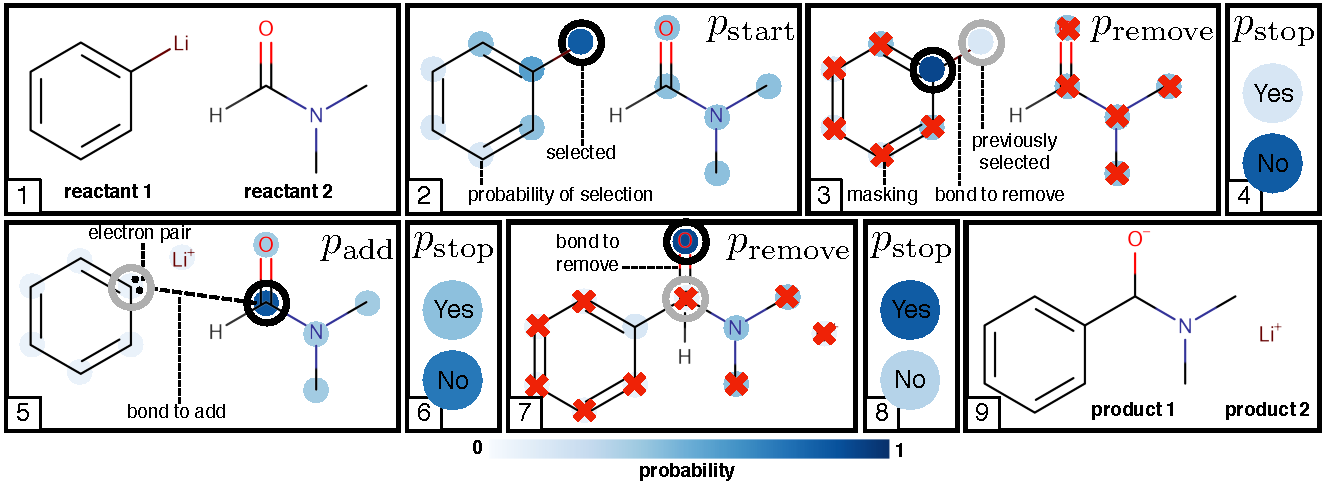
\includegraphics[width=\textwidth]{reaction_model_blue}
\caption{A visualization of the actions taken by the model to sequentially perform a simple reaction.}
\label{fig:reaction_model}
\end{figure*}



In this section we define a probabilistic model that describes the flow of movement of electrons that define an elementary heterolytic reaction.
We represent a set of molecules as a graph $\moleculeSet$, with atoms $\Ac$ as vertices and bonds $\Bc$ as edges;
each connected component of the graph defines an individual molecule.
Each atom $\Ac$ includes a set of features \todo[]{LIST THESE},
and each bond $\Bc$ can be a single bond, double bond, or triple bond \todo[]{aromatic bonds?}.

Given an initial set of reactant molecules $\moleculeSet_0$ and a set of reagent molecules $\moleculeSet_r$, 
our model defines a conditional distribution over a sequence of atoms $\electronPath_{0:T} = (a_0, a_1, \ldots, a_T)$,
which fully characterizes the electron path.
This electron path in turn deterministically defines both a final product $\moleculeSet_{T}$, 
denoting the outcome of the reaction,
as well as a sequence of intermediate products $\moleculeSet_t$, for $t = 1,\dots,T-1$,
which correspond to the state of the graph after the first $t$ steps in the subsequence $\electronPath_{0:t} = (a_0, \dots, a_t)$ are applied to the initial $\moleculeSet_t$.


We propose to learn a parameterized distribution $p_\theta( \electronPath_{0:T} \mid \moleculeSet_0, \moleculeSet_r)$ over electron movements. 
We begin by describing the generative process %(i.e., the forward pass) 
of $p_\theta$, and then describe how to train the model parameters.


\subsection{Generative process}

The joint probability of an electron path can be factorized into a product of distributions
defining the probability $p(a_0 \mid \initialAndReactants)$ of the initial state $a_0$ given the reactants and reagents, 
the conditional probability $p(a_t \mid \moleculeSet_t, t)$ \todo[]{maybe somehow refer to "bond type" instead of $t$?} of next state $a_t$ given the intermediate products $\moleculeSet_t$ for $t > 0$,
and the probability $p(s_t \mid \moleculeSet_t)$ that the reaction terminates with final product $\moleculeSet_t$.

%The distribution over electron paths can be factorized as follows:
%%\begin{align}
%%p_\theta(\electronPath \mid \moleculeSet_0) = p_\theta(s_{0}' \mid \moleculeSet_0) p_\theta(a_{0} \mid \moleculeSet_0) \prod_{t=1}^{T-1} \left( p_\theta(a_{t} \mid a_{t-1}, \Mc_{t-1} ) p_\theta(s_{0}' \mid \moleculeSet_0) \right) p_\theta(a_{T} \mid a_{T}, \Mc_{T-1} ) p_\theta(s_{T} \mid \moleculeSet_T) \nonumber
%%\end{align}
%
%\begin{align*}
%p(\electronPath_{0:T} \mid \initialAndReactants) = &
% \quad 
% p(s_0' \mid \initialAndReactants)
% p(a_0 \mid \initialAndReactants)
% \prod_{t=1}^{T} \Big[ 
% 	p(s_t' \mid \initialAndReactants, \electronPath_{0:t-1})
% 	p(a_t \mid \initialAndReactants, \electronPath_{0:t-1} ) 
% \Big] \\
% & \times p(s_{T+1} \mid  \initialAndReactants, \electronPath_{0:T} )
%\end{align*}

%\improvement[]{this part a bit messy}
%Where $p(s_{t})$ is the probability of stopping the path before picking the $t^{\text{th}}$ action, $p(s_{t}')$ of continuing.


In practice we assume that the probability of an action depends only on (i) the intermediate molecule formed by the action path up to that point, (ii) the previous action taken (indicating where the free pair of electrons are) and (iii) the point of time through the path, indicating whether we are on an add or remove bond step. 
We further make the simplifying assumption that the stop probability and the actions after $a_0$ do not depend on the reagents. This leads to a model with dependency structure
\begin{align}
p_\theta(\electronPath_{0:T} \mid \moleculeSet_0, \moleculeSet_r) 
&=
       p(a_0 \mid \moleculeSet_0, \moleculeSet_r)
       p(s'_0 \mid \moleculeSet_0)
\prod_{t=1}^{T} 
	p(a_t \mid \moleculeSet_{t+1}, a_{t-1}, t)
	p(s_{t+1} \mid \moleculeSet_{t+1}),
\label{eq:jointprob}
\end{align}
where we have defined $p(s'_t \mid \moleculeSet_t) \equiv 1 - p(s_t \mid \moleculeSet_t)$ to be the probability of {\em continuing} a reaction given the current molecule set $\moleculeSet_t$\improvement[]{this part still a bit messy}.
%
%
%%% THIS IS THE PREVIOUS VERSION:
%\begin{align*}
%p_\theta(\electronPath_{0:T} \mid \moleculeSet_0, \moleculeSet_r) = &
% \quad \continueProb{0}{0}
%       p(a_0 \mid \moleculeSet_0, \moleculeSet_r)
%       p(a_1 \mid \moleculeSet_0, a_0) \\
%       & \times \prod_{t=2}^{T} \Big[
%              \continueProb{t}{\electronPath_{0:t-1}}
%              \actionProb{t}
%       \Big] \\
%       & \times p(s_{T+1} \mid \moleculeSet_{\electronPath_{0:T}})
%\end{align*}
%
Note that you cannot stop after one action, as you have to pick up a complete electron pair;
however, it is possible to stop prior to selecting a first atom $a_0$, indicating that no reaction would take place.
Given any particular selected atom $a_t$ which extends the reaction path, we can deterministically update the previous molecular graph $M_{t}$ to produce the next set of (intermediate) products $M_{t+1}$.

As described in the previous section, if the three reaction assumptions above hold, then there are two types of electron movements that alternate: 
(1) movement that \emph{removes an existing bond}, and 
(2) movement that \emph{adds a new bond}. 
We can generalize assumption 3 by defining that atoms with free electrons have a self-bond. 
Thus, all reactions start by first selecting an atom, removing a bond (between two different atoms, or a self-bond), and then alternately adding and removing bond;
we can determine whether a particular step is an add step or remove step by inspecting $t$.
Note that $\moleculeSet_1 = \moleculeSet_0$, as the initial action of selecting $a_0$ does not remove or form any bonds\todo{maybe put this somewhere else}.

Each of the conditional probabilities in Eq.~\eqref{eq:jointprob} is parameterized by a neural network:
for each stage the network takes the current intermediate product graph, 
along with the previous action and the reagents if relevant, 
to compute a probability distribution over next possible actions (i.e., selecting a particular atom, or stopping).
These architectures will be described in the following section.

Figure~\ref{fig:reaction_model} shows a simple example reaction, which demonstrates all the critical features of the model.
The first subfigure shows two reactants, which we assume will react (i.e.\ $s_0 = 1$).
Subsequent subfigures show the network picking an initial atom to begin the electron path,
and then iteratively selecting atoms for removing and adding bonds, potentially stopping after each action.
Masking at each add and remove step can reduce the total number of possibilities: 
for example, it is not possible to remove a bond which does not exist in the graph $\moleculeSet_t$.
\todo[]{walk through figure. do we want to that HERE, or in the caption? or elsewhere?}

\subsection{Computing atom and molecule features}


%\unsure[]{This part is not quite right. We currently have a f second, although Im training models that no longer have this}
As each of the remove-bond, add-bond, and start-atom steps represent probability distributions over a fixed set of atoms in the intermediate product graph $M_t$, they are specified in similar ways.
Essential to each is an appropriate representation of the molecule graph $M_t$.
We define a function $f_{\Ac} (\moleculeSet)$ which returns a set of $d$-dimensional feature vectors, 
one for each vertex (atom) $\Ac$ in the graph $\moleculeSet$.
% so that $f_{\Ac}(\moleculeSet) \subseteq \mathbb{R}^{|\Ac| \times d}$. 
In general $f_{\Ac}$ could be any deep graph model that uses the graph structure of $\Mc_t$ to get graph-isomorphic node features, usually via message-passing techniques \citep{gilmer2017neural}. 
We choose to use Gated Graph Neural Network message functions \citep{li2016gated},
which take our original set of vertex features for each atom $\Ac$ and compute new representations that
additionally embed information about the atom in relation to other atoms in its neighborhood in the graph\todo[]{this is hokey, i'm sorry, please delete}.

Using these atom features, we can define the conditional distribution for the remove, add, and start steps.
To produce probabilities over the individual atoms given the atom features and the previous action $a_{t-1}$,
both are input to a function $f_{\textrm{remove}}$ which is input to a softmax function and then masked, with
\begin{align}
\Hb_{\Ac} \;&= f_{\Ac}(\moleculeSet_t) \label{eq:rem_atom} \\
%\Hb_{\Bc} \;&= f_{\Bc}(\Mc_t, \Hb_{\Ac}) \label{eq:rem_bond} \\
p(a_t \mid \moleculeSet_{t}, a_{t-1}) 
\;&\propto \beta_{\mathrm{remove}}(a_{t-1}, \cdot) \  \mathrm{softmax}(f_{\textrm{remove}}(\Hb_{\Ac}, a_{t-1})). \label{eq:rem_prob}
\end{align}
The masks are binary values with $\beta_{\mathrm{remove}}({a_{t-1}, a}) = 1$ if the bond $(a_{t-1}, a)$ exists in the molecule set $\moleculeSet_t$.
In this manner, the previous action can be used to mask the possible probabilities, as it is structurally impossible to remove a bond which does not exist.
The function $f_{\textrm{remove}}$ is defined as a neural network with a single hidden layer.
\todo[]{is this correct? network architecture details are missing everywhere...}
When removing the initial bond we also allow the removal of self bonds.


%Recall that $\Mc_t$ is a deterministic function of $\Mc_0$ and $a_{0:t-1}$.
%
%Function $f_{\Ac}$ in eq.~\eqref{eq:rem_atom} takes a molecular graph and for each atom outputs a set of $d$-dimensional atom features, so that $\Hb_{\Ac} \subseteq \mathcal{R}^{|\Ac| \times d}$. 
%To produce probabilities over the individual atoms given the atom features $\Hb_{\Ac}$ and the previous action $a_{t-1}$, we introduce a function $f_{\textrm{remove}}$, followed by a $\mbox{softmax}$ function.
%The previous action $a_{t-1}$ is used to mask the resulting probabilities as 
%\improvement[]{Maybe confusing having this and also the eqn 2. above. Maybe should merge.}
%
%\begin{align}
%p(a \mid \moleculeSet_t, a_{t-1})) \propto 
%\begin{cases}
%\mbox{softmax}(f_{\textrm{remove}}(\Hb_{\Ac})) & \mbox{if bond } (a_{t-1},a) \mbox{ exists in } \moleculeSet_{t} \\
%0 & \mbox{otherwise}. \nonumber
%\end{cases}
%%\label{eq:rem_prob}
%%In Eq.~\eqref{eq:rem_prob}
%\end{align}

\improvement[]{add time indexing to the node features}
For an add-bond step, we again use Eq.~\eqref{eq:rem_atom} to obtain atom features $\Hb_{\Ac}$ and use a different function $f_{\textrm{add}}$ to produce probabilities for adding bonds as 
\begin{align}
p(a_t \mid \Mc_t, a_{t-1}) \propto \beta_{\mathrm{add}}(a_{t-1}, \cdot) \ \mbox{softmax}(f_{\textrm{add}}(\Hb_{\Ac}), a_{t-1})
% \begin{align}
% \Hb_{\Ac} \;&= f_{\Ac}(\Mc_t) \label{eq:add_atom}  \\
% p(a_t \mid a_{0:t-1}, \Mc_0) \;&= \mbox{softmax}(f_{\textrm{add}}(\Hb_{\Ac}, a_{t-1})). \label{eq:add_prob}
 \end{align}
%The primary difference here is instead of a distribution over existing bonds, the distribution in eq.~\eqref{eq:add_prob} is over all possible atoms $\Ac$ (and a `null' action), as a bond may possibly form between any two atoms. 
The primary difference here is in the choice of mask:
we again use the previous action $a_{t-1}$ to mask probabilities, 
although here we only mask out the probability of adding a self-bond to the current atom
(that is, $\beta_{\mathrm{add}}(a_{t-1}, a) = 1$ for all $a \neq a_{t-1}$).

\highlight{[BP: i don't understand this next paragraph...]} We calculate stop probabilities as 
\begin{align}
p(s_t \mid \moleculeSet_{\electronPath_{0:t-1}} ) = \mbox{sigmoid}(\fStop(\Hb_{\Ac})).
\end{align}
Here $\fStop$ is similar to the readout functions in \citet[eq. 4]{gilmer2017neural}. In particular,
$\fStop(\Hb_{\Ac}) = k \left( \sum_{v \in \Ac} \left[ \mbox{sigmoid}(i(\Hb_{\Ac,v})) \cdot j(\Hb_{\Ac,v}) \right] \right)$.
In which $i$, $j$ and $k$ are functions parameterized by neural networks, with $k$ projecting the graph down to one dimension \improvement[]{well actually just linear layers... Two things here 1. slightly different to Gilmer. 2. When doing reagents forget to mask out empty nodes when doing the sum, so they will have whatever biases the network learns...}.

Finally, in order to select the starting atom of a path we propose to model the initial probability as 
\begin{align}
p(a_0 \mid \moleculeSet_0, \moleculeSet_r) = \mbox{softmax}(f_{\textrm{start}}(\Hb_{\Ac}, \fReagEmbed(\moleculeSet_r))).
\end{align}
There is no masking used for this step. 
Here $\fReagEmbed$ returns an embedding of the reagents.
This is created by (i) computing node features for the reagents, using $f_{\Ac}$, then (ii) calculating a graph embedding, by using a similar function to $\fStop$ but one which calculates multidimensional features;
finally (iii) these features for each reagent are summed  to produce a final embedding that is invariant to the ordering of reagents.

\paragraph{Training}
We can learn the parameters $\theta$ of the functions $\fModules$, by maximizing the likelihood of the true path $\log p_\theta(\electronPath_{0:T} \mid \moleculeSet_0, \moleculeSet_r)$.
%\begin{align*}
%%  \min_{\fModules}
%\min_{\theta}
%    & - \log \continueProb{0}{0} - \log p(a_0 \mid \moleculeSet_0, \moleculeSet_r)  - \log p(a_1 \mid \moleculeSet_0, a^*_0) \\
%	& - \sum_{t=2}^{T} \log \Big[ \continueProb{t}{\electronPath_{0:t-1}^*} \actionProb[*]{t} \Big] \\
%    & - \log p(s_{T+1} \mid \moleculeSet_{\electronPath_{0:T}^*})
%\end{align*}
This is evaluated by using a known true electron path $a_t^\star$ and intermediate products $\moleculeSet_t^\star$ extracted from training data,
rather than on simulated values, 
so that we are using teacher forcing \citep{williams1989learning} during training\todo[]{is this "teacher forcing"? I think this is just plain maximum likelihood estimation of the individual modules...}. 
This allows us to train on all stages of the reaction at once.

\paragraph{Sampling}
Once trained we can sample chemically-valid paths from our model using beam search.  This is procedure is described in Algorithm~\ref{algo:valid_path}\todo[]{briefly describe beam search}. 




\newcommand{\cProbCont}{\texttt{calc\_prob\_continue}}
\newcommand{\cProbAct}{\texttt{calc\_prob\_action}}
\newcommand{\cProbInitial}{\texttt{calc\_prob\_initial}}
\newcommand{\removeFlag}{F_\textrm{remove}}

\newcommand{\outputPool}{\hat{\Pc}}
\newcommand{\cPath}{\rho}
\newcommand{\lProb}{p_{\textrm{path}}}


%\begin{wrapfigure}{R}{0.5\textwidth}
\begin{figure}
\begin{minipage}{1.\textwidth}
\begin{algorithm}[H]
  \caption{Predicting electron paths at test time.}
  {\bf Input:}~~Molecule $\Mc_0$ (consisting of atoms $\Ac$), reagents $\Mc_r$ , beam width $K$, time steps $T^\mathrm{max}$
  
  \begin{algorithmic}[1]
  	% Set up pool of completed paths to sort later
  	\STATE $\outputPool = \{\left( \emptyset, \log (1 - \cProbCont(\Mc_0)) \right) \}$  \COMMENT{This set will store all completed paths.}
  	\STATE $\removeFlag \!=\!1$ \COMMENT{remove flag}
  	
  	% Pick the first action.\\
  	\STATE
	\STATE $\hat{\Bc} = \emptyset$.  \COMMENT{This set will store all possible open paths. Cleared at start of each timestep.}	
	\FORALL{$v \in \Ac$} 
		\STATE $ \cPath = (v)$
		\STATE $ \lProb = \log \cProbCont(\Mc_0) + \log \cProbInitial(v, \moleculeSet_0, \moleculeSet_r)$
		\STATE $\hat{\Bc} = \hat{\Bc} \cup \{\left(\cPath, \lProb \right)\}$
	\ENDFOR
	\STATE  $\Bc_{0} = \texttt{pick\_topK\_actions}(\hat{\Bc})$ \COMMENT{We filter down to the top K most promising actions.}
	
	% Then we evaluate the next stages.
	\STATE
	\FOR{t in $(1, \ldots, T^\mathrm{max})$}
		\STATE $\hat{\Bc} = \emptyset $ 
				
		% We take all the previous top K open paths from the previous step...
		\FORALL{$(\cPath, \lProb) \in \Bc_{t-1}$} 
			
			% We evaluate their stop probability at that point and add these stopped version to the completed pool.
			\STATE $\Mc_\cPath = \texttt{calc\_intermediate\_mol}(\Mc_0, \cPath)$
			\STATE $p_c = \cProbCont(\Mc_\cPath)$
			\STATE $\hat{\Pc} = \hat{\Pc} \cup \{(\cPath, \lProb + \log (1 - p_c))\}$
			
			% We then see what would happen if we continued and picked another action.
			\FORALL{$v \in \Ac$}
				\STATE $\cPath' = \cPath^\frown (v)$ \COMMENT{New proposed path is concatenation of old path with new node.}

				\STATE $v_{t-1} = $ last element of $\cPath$
				\STATE $\hat{\Bc} = \hat{\Bc} \cup \{(\cPath' , \lProb + \log p_c + \log \cProbAct(v, \Mc_\cPath, v_{t-1}, \removeFlag) )\}$
			\ENDFOR
		\ENDFOR
		
		% We next prune down the search space for next iteration to our beam width.
		\STATE  $\Bc_{t} = \texttt{pick\_topK\_actions}(\hat{\Bc})$ 
		
		% We indicate that the next step will be opposite step:
		\STATE $\removeFlag = \removeFlag + 1 \mod 2$. \COMMENT{If on add step change to remove and vice versa.}
	\ENDFOR
	
  % Finally we sort the pool and we are done
  \STATE
  \STATE $\outputPool = \texttt{sort\_on\_prob}(\outputPool)$
  \end{algorithmic}
  {\bf Output:}~~Valid completed paths and their respective probabilities, sorted by the latter, ~$\outputPool$
  \label{algo:valid_path}
\end{algorithm}
\end{minipage}
%\end{wrapfigure}
\end{figure}
